\documentclass[11pt,a4]{article}
\usepackage{german}
\usepackage{graphicx,parskip,times,amsfonts,amsmath}

\begin{document}
 \tableofcontents
% Das erzeugt einen Kommentar. Die Inhalte werden nicht �bersetzt. Der Befehl \tableofcontents erzeugt automatisch ein Inhaltsverzeichnis.
% \newpage f�gt eine neue Seite ein%

%\newpage
\section{Introduction}
Dann schreiben wir Text einfach so wie immer. Das ist ein Beispieltext. Der Zeilenumbruch ist egal,
 der   Abstand zwischen W\"{o}rtern ist egal, LaTex trennt automatisch und  f\"{u}gt
 auch automatisch Umbr\"{u}che ein. 
\section{So erzeugt man ein LaTeX Dokument}
\begin{itemize}
\item Anlegen einer Datei mit der Endung .tex, z.B. Test.tex
\item Jede LaTeX Datei  beginnt mit einem documentclass Befehl, z.B.: \\
$\backslash$documentclass[11pt]\{article\} \\
und weiteren definitionen, z.B. $\backslash$usepackage\{german\}.
Das eigentliche Dokument beginnt mit
$\backslash$begin\{document\}. Es folgt der Text und man endet das Document mit einem $\backslash$end\{document\}.
\end{itemize}
Die Aufz\"{a}hlung erzeugt man mit 
$\backslash$begin\{itemize\}, gefolgt von den Items mit $\backslash$item und beendet diese mit $\backslash$end\{itemize\}.
So und dann sind wir wieder im normalen Modus.

\subsection{\"{U}berschrift level 2}
Mit $\backslash$section erzeugt man ein Kapitel, mit $\backslash$subsection ein Unterkapitel usw. Umlaute und Symbole erzeugt man indem man die Symbolleiste des WinEdt einblendet und auf die Symbole klickt, z.B.  f\"{u}gt {\oe}{\ae}{\aa}{\o}{\l}{\i}?`\"{\i}\"{O}\c{C}\`{O}\t{ }ein. Au{\ss}erdem muss man bei dem {\ss} aufpassen und bei anderen Zeichen, die ein Befehl in LaTeX sein k\"{o}nnten. Und dann setzen wir noch ein nettes Bild auf die Seite:

\subsection{Math Modus}
Formeln sind oft auch in naturwissenschaftlichen Texten enthalten. Aber meistens arbeiten diese Profs sowieso mit LaTeX. Aber so schwer ist das auch nicht. Kurze Formeln beginnen und enden mit einem \$ . Dazwischen f\"{u}gt man die Zeichen mit dem WinEdt ein, so z.B. $\sum \beta\gamma\epsilon\psi \sinh \! \quad  $ usw.

\subsubsection{Abbildung}
Abbildungen f\"{u}gt man einfach ein. Dazu m\"{u}ssen die Dateien im pdf, jpg, jpeg oder png Format vorliegen. Man bindet die Dateinamen ohne Endungen ein:   
\begin{figure}[htb]
\begin{center}
 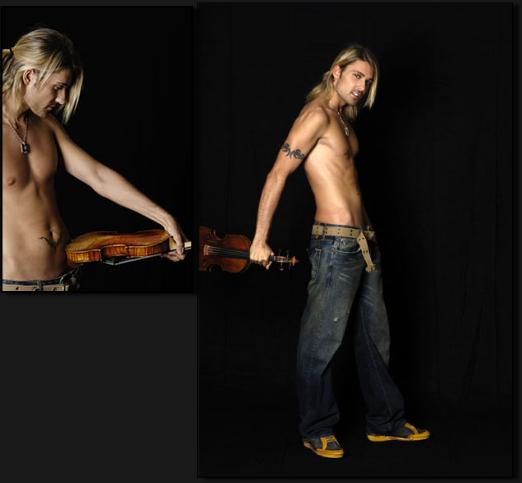
\includegraphics[width=8cm]{davidgarrett2200b}
  \caption{Ein begnadeter Geiger}
  \end{center}
\end{figure}
 
 \end{document} 